\subsection{Esquema general}
El sistema propuesto tiene como objetivo optimizar el uso del recurso hídrico en los cultivos de plantas del Vivero Michita. A través de la implementación de sensores y lógica difusa, se logrará un riego preciso y adaptativo. A continuación, se detallan en la Figura \ref{fig:esquema_general} las etapas claves del sistema:

\begin{figure}[H]
    \centering
    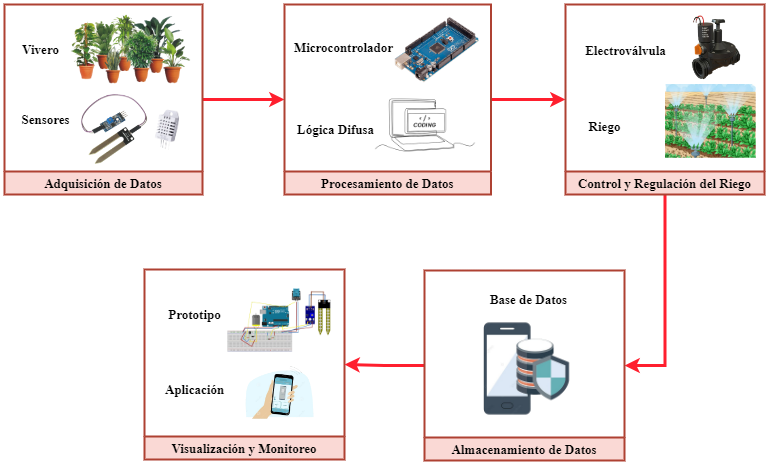
\includegraphics[width=15cm,height=13cm,keepaspectratio]{resources/images/esquema-general.png}
    \caption{Esquema General}\label{fig:esquema_general}
\end{figure}

\subsection*{Etapa 1: Adquisición de Datos}
El sistema inicia adquiriendo datos en tiempo real mediante sensores de humedad del suelo, temperatura y ambiente instalados en el vivero. Estos sensores proporcionan información crucial sobre las condiciones del suelo y las necesidades hídricas de las plantas. Todos estos datos son esenciales para el siguiente proceso.

\subsection*{Etapa 2: Procesamiento de Datos}
En esta etapa, los datos recopilados se procesan mediante un algoritmo diseñado para determinar la cantidad óptima de agua necesaria para cada área de cultivo. Se utiliza la lógica difusa para adaptar las estrategias de riego a los cambios ambientales, considerando factores como sensores de humedad del suelo, temperatura y ambiente. Este procesamiento permite una toma de decisiones más precisa y eficiente en el manejo del agua en el vivero para cada categoría de planta.

\subsection*{Etapa 3: Control y Regulación del Riego}
Una vez procesados, los resultados determinados por el algoritmo se utilizan para ajustar el riego de manera óptima. El sistema controla las válvulas de riego para distribuir el agua de acuerdo con las necesidades específicas de cada zona del vivero, garantizando un uso eficiente del recurso hídrico y proporcionando el cuidado adecuado a las plantas en cada área de cultivo.

\subsection*{Etapa 4: Almacenamiento de Datos}
Los registros de riego y los datos procesados se almacenan en una base de datos para su posterior análisis. Este almacenamiento permite evaluar el desempeño del sistema a lo largo del tiempo y facilita la identificación de áreas de mejora. El análisis de datos acumulados proporciona información valiosa para optimizar el funcionamiento del sistema y realizar mejoras continuas en su rendimiento.

\subsection*{Etapa 5: Visualización y Monitoreo}
Los responsables del vivero tienen acceso a una interfaz de visualización que muestra el estado de las áreas de cultivo y el progreso de la humedad del suelo en tiempo real. Esta visualización incluye el historial de riego que ayudan a tomar decisiones informadas sobre el manejo del agua y garantizar un uso eficiente del recurso.
